\subsection{快速傅里叶变换}

考虑 DFT 的计算公式
\begin{align*}
    X(k) = \DFT{x(n)} = \sum_{n = 0}^{N - 1}x(n)W_N^{nk},
\end{align*}
其中 $k = 0, 1, \cdots, N - 1$。
每计算一个 $X(k)$,都需要 $N$ 次复数乘法和 $N - 1$ 次复数加法。
因此,计算出所有的 $X(k)$ 的时间复杂度为 $O(N^2)$。

尽管预先计算出 $W_N^{nk}$ 的值可以减少计算量,但是仍然需要 $O(N^2)$ 的时间。
因此,我们需要寻找一种更快的计算方法。这就是\bd{快速傅里叶变换}(FFT)。

\subsubsection{快速傅里叶变换的原理}

经过周期性与对称性简化之后,容易发现 DFT 运算中存在着不必要的重复计算。
避免这种重复,是简化运算的关键。FFT 利用了 $W_N$ 的周期性和对称性,
将 $N$ 点 DFT 分解为 $N/2$ 点 DFT,$N/4$ 点 DFT,……,$2$ 点 DFT,
从而实现了 DFT 的快速运算。

\begin{property}[$W_N^{nk}$ 的性质]
    记 $W_N = \mathe^{-2\pi\mathi / N}$,则有
    \begin{align*}
        W_N^{nk} = W_N^{nk \bmod N}, \\
        W_N^{nk + N/2} = -W_N^{nk}.
    \end{align*}
\end{property}

\begin{proof}
    由于 $W_N = \mathe^{-2\pi\mathi / N}$,故 $W_N^N = \mathe^{-2\pi\mathi} = 1$。
    因此,$W_N^{nk} = W_N^{nk \bmod N}$。又因为 $W_N^{N/2} = \mathe^{-\pi\mathi} = -1$,
    故 $W_N^{nk + N/2} = -W_N^{nk}$。命题得证。
\end{proof}

\begin{theorem}
    设 $N$ 为 $2$ 的整数次幂,$N = 2^M$。对于 $N$ 点序列 $x(n)$,其 DFT 为 $X(k)$。
    则 $X(k)$ 可以分解为 $N/2$ 点序列 $G(k)$ 和 $H(k)$ 的 DFT 的线性组合。
    其中 $G(k)$ 是 $g(r) = x(2r)$ 的 $N/2$ 点 DFT,$H(k)$
    是 $h(r) = x(2r + 1)$ 的 $N/2$ 点 DFT,$r = 0, 1, \cdots, N/2 - 1$。
\end{theorem}

\begin{proof}
    将 $X(k)$ 分为偶数项和奇数项,即
    \begin{align*}
        X(k) & = \sum_{r = 0}^{N/2 - 1}x(2r)W_N^{(2r)k}
            + \sum_{r = 0}^{N/2 - 1}x(2r + 1)W_N^{(2r + 1)k} \\
        & = \sum_{r = 0}^{N/2 - 1}x(2r)W_{N/2}^{rk}
            + W_N^k\sum_{r = 0}^{N/2 - 1}x(2r + 1)W_{N/2}^{rk}.
    \end{align*}
    由于 $g(r) = x(2r), h(r) = x(2r + 1)$,其中 $r = 0, 1, \cdots, N/2 - 1$,故
    \begin{align*}
        \begin{cases}
            \sum_{r = 0}^{N/2 - 1}x(2r)W_{N/2}^{rk}
                = \sum_{r = 0}^{N/2 - 1}g(r)W_{N/2}^{rk} = G(k), \\
            \sum_{r = 0}^{N/2 - 1}x(2r + 1)W_{N/2}^{rk}
                = \sum_{r = 0}^{N/2 - 1}h(r)W_{N/2}^{rk} = H(k),
        \end{cases}
    \end{align*}
    其中 $k = 0, 1, \cdots, N/2 - 1$。因此
    \begin{align*}
        X(k) = G(k) + W_N^kH(k), \quad k = 0, 1, \cdots, N/2 - 1.
    \end{align*}
    再考虑后半部分,
    \begin{align*}
        X\left(\frac{N}{2} + k\right) & = \sum_{r = 0}^{N/2 - 1}x(2r)W_{N/2}^{r\left(\frac{N}{2} + k\right)}
            + W_N^{k + N/2}\sum_{r = 0}^{N/2 - 1}x(2r + 1)W_{N/2}^{r\left(\frac{N}{2} + k\right)} \\
        & = \sum_{r = 0}^{N/2 - 1}x(2r)W_{N/2}^{rk}
            - W_N^k\sum_{r = 0}^{N/2 - 1}x(2r + 1)W_{N/2}^{rk} \\
        & = \sum_{r = 0}^{N/2 - 1}g(r)W_{N/2}^{rk}
            - W_N^k\sum_{r = 0}^{N/2 - 1}h(r)W_{N/2}^{rk} \\
        & = G(k) - W_N^kH(k), \quad k = 0, 1, \cdots, N/2 - 1.
    \end{align*}
    综上所述,
    \begin{align*}
        X(k) = G(k) + W_N^kH(k), \quad X\left(\frac{N}{2} + k\right) = G(k) - W_N^kH(k),
    \end{align*}
    其中 $k = 0, 1, \cdots, N/2 - 1$。
    命题得证。
\end{proof}

\begin{exercise}
    本课介绍了 DFT 的快速算法 FFT。相应地,可将 $N$ 点 IDFT 运算递归地分解
    为 $N/2$ 点,$N/4$ 点,……,$2$ 点 IDFT 运算,从而实现 IDFT 的快速运算。

    设序列 $X(k)$ 的长度为 $N$,$N$ 为
    偶数,$X(k)$ 的 $N$ 点 IDFT 为 $x(n)$。$G(k)$ 是 $X(k)$ 中
    下标为偶数的元素组成的子序列,$H(k)$ 是 $X(k)$ 中下标为奇数的元素
    组成的子序列,它们的长度是 $N/2$,对应的 $N/2$ 点 IDFT 分别
    是 $g(n)$ 和 $h(n)$。试用 $g(n)$ 和 $h(n)$ 表示 $x(n)$。
\end{exercise}

\begin{solution}
    IDFT 的定义为
    \begin{align*}
        x(n) = \frac{1}{N}\sum_{k = 0}^{N - 1}X(k)W_N^{-kn},
    \end{align*}
    可以将其分为两组,
    \begin{align*}
        x(n) & = \frac{1}{N}\sum_{k = 0}^{N/2 - 1}X(2k)W_N^{-2kn}
            + \frac{1}{N}\sum_{k = 0}^{N/2 - 1}X(2k + 1)W_N^{-(2k + 1)n} \\
        & = \frac{1}{N}\sum_{k = 0}^{N/2 - 1}G(k)W_{N/2}^{-kn}
            + \frac{W_N^{-n}}{N}\sum_{k = 0}^{N/2 - 1}H(k)W_{N/2}^{-kn}.
    \end{align*}
    由于 $G(k) = X(2k), H(k) = X(2k + 1)$,其中 $k = 0, 1, \cdots, N / 2 - 1$,故
    \begin{align*}
        \begin{cases}
            \sum_{k = 0}^{N/2 - 1}X(2k)W_{N/2}^{-kn}
                = \sum_{k = 0}^{N/2 - 1}G(r)W_{N/2}^{-kn} = \frac{N}{2}g(n), \\
            \sum_{k = 0}^{N/2 - 1}X(2k + 1)W_{N/2}^{-kn}
                = \sum_{k = 0}^{N/2 - 1}H(r)W_{N/2}^{-kn} = \frac{N}{2}h(n),
        \end{cases}
    \end{align*}
    其中 $n = 0, 1, \cdots, N/2 - 1$。因此
    \begin{align*}
        x(n) = \frac{1}{2}\left(g(n) + W_N^{-n}h(n)\right), \quad n = 0, 1, \cdots, N / 2 - 1.
    \end{align*}
    再考虑后半部分,
    \begin{align*}
        x\left(\frac{N}{2} + n\right) & = \frac{1}{N}\sum_{k = 0}^{N/2 - 1}X(2k)W_{N/2}^{-k\left(\frac{N}{2} + n\right)}
            + \frac{W_N^{-\left(\frac{N}{2} + n\right)}}{N}\sum_{k = 0}^{N/2 - 1}X(2k + 1)W_{N/2}^{-k\left(\frac{N}{2} + n\right)} \\
        & = \frac{1}{N}\sum_{k = 0}^{N/2 - 1}X(2k)W_{N/2}^{-kn}
            - \frac{W_N^{-n}}{N}\sum_{k = 0}^{N/2 - 1}X(2k + 1)W_{N/2}^{-kn} \\
        & = \frac{1}{N}\sum_{k = 0}^{N/2 - 1}G(k)W_{N/2}^{-kn}
            - \frac{W_N^{-n}}{N}\sum_{k = 0}^{N/2 - 1}H(k)W_{N/2}^{-kn} \\
        & = \frac{1}{2}\left(g(n) - W_N^{-n}h(n)\right), \quad n = 0, 1, \cdots, N / 2 - 1.
    \end{align*}
    综上所述,
    \begin{align*}
        x(n) = \frac{1}{2}\left(g(n) + W_N^{-n}h(n)\right),
            \quad x\left(\frac{N}{2} + n\right) = \frac{1}{2}\left(g(n) - W_N^{-n}h(n)\right),
    \end{align*}
    其中 $n = 0, 1, \cdots, N / 2 - 1$。
\end{solution}

\subsubsection{快速傅里叶变换的时间复杂度}

\begin{theorem}
    设 $N$ 为 $2$ 的整数次幂,$N = 2^M$。对于 $N$ 点序列 $x(n)$,其 DFT 为 $X(k)$。
    则 FFT 的时间复杂度为 $O(N\log N)$。如图 \ref{fig:FFT_calc} 所示。
    \begin{figure}[H]
        \centering
        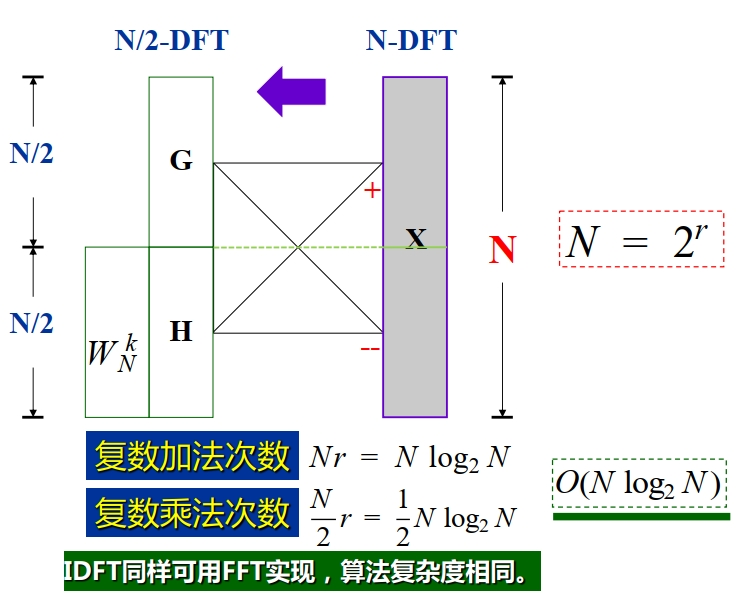
\includegraphics[width = 0.6\textwidth]{chap3/img/FFT_calc.png}
        \caption{FFT 的计算流程}
        \label{fig:FFT_calc}
    \end{figure}
\end{theorem}
